\documentclass[a4paper,10pt,DIV15]{scrartcl}
\usepackage[psamsfonts]{amssymb}
\usepackage{amsmath}
%\usepackage{latexsym}
\usepackage{theorem}


\usepackage{fontspec,xunicode,xltxtra}
\usepackage[ngerman]{babel}
\selectlanguage{ngerman}


\usepackage[svgnames,hyperref]{xcolor} %color definitions
%\usepackage{tikz}
%\usetikzlibrary{shadows}
%\usetikzlibrary{fit}
%\usetikzlibrary{shapes}
%\usetikzlibrary{backgrounds}


\usepackage{mcode}
%\usepackage{pstricks,pst-node,pst-text,pst-3d}
\parindent0cm % Abs�tze nicht einr�cken 

%---- neue Umgebung f�r Aufgaben
\theoremstyle{break}
\theoremheaderfont{\Large \bf}
\theorembodyfont{\normalfont}


% Definieren einer neuen Farbe
\definecolor{light-gray}{gray}{.9}

\newcounter{zaehler}     % neuen Z�hler einf�hren
\stepcounter{zaehler}    % Z�hler einen hochz�hlen

\newenvironment{aufg}%
%---- Header
{\begin{samepage}
\colorbox{light-gray}{                         % Box in gray
 \makebox[\textwidth]{                           % Box in linewidth
\textbf{Aufgabe} \arabic{zaehler} :}}\\[0.1cm]       % Header
%\begin{minipage}{0.5cm} \end{minipage}    % Insert 0.5cm
\begin{minipage}{\textwidth}}
%-----  foot
{\end{minipage} \nopagebreak %\begin{minipage}{1cm} \end{minipage}
\\[0.1cm] 
%\begin{minipage}{0.1cm} \end{minipage} 
%\hrulefill \begin{minipage}{1cm} \end{minipage}\\[1cm]  
\stepcounter{zaehler}                           % increase counter
 \end{samepage}%
}

%-------------------------------------------------------------------------------
\begin{document}
%-------------------------------------------------------------------------------

%--------------------------------------------------- Header
\begin{center}
\textbf{\LARGE Einf\"uhrung in MATLAB }\\
\end{center}
\begin{minipage}{6cm}
Dr. J. Schulz\\
\end{minipage}\hfill
\begin{minipage}{2cm}
\textbf{Einheit 3}\\
%30.07.2007
\end{minipage}\\[1cm]

\begin{aufg}
\begin{itemize}
\item Interpolieren Sie an den durch \lstinline!x=linspace(-5,5,13)! gegebenen Stellen  die Funktion $f(x):=x^2\exp(-|x|)$.
\item Berechnen Sie approximativ den maximalen Fehler zwischen $f$ und
  ihrer Interpolierenden auf $[-5,5]$. 
(Hinweis: Befehl \lstinline!max!)
\item Ändern Sie den Vektor der Stützstellen
  \lstinline!x=linspace(-5,5,13)!, so dass 
\[ x_i = - 5 \cos(\pi (i-1)/12), \quad i=1, \dots , 13. \]
Berechnen Sie erneut den maximalen Fehler.
\item Betrachten Sie auch die Stützstellen
\[ x_i = - 5 \cos(\pi (i-1)/49), \quad i=1, \dots , 50. \] 
\end{itemize}
\end{aufg}

%-----------------------------------------------------------------------------------

\begin{aufg}
Schreiben Sie ein Programm, dass zu einem gegebenen $a>0$ die
  Funktion
\[ f(x):= 1/(x^2+a) \]
auf dem Intervall $[-3,3]$ plottet. 

%Erstellen Sie daraus eine Animation f\"ur $a \in [0,5]$.
\end{aufg}


%-----------------------------------------------------------------------------------
\begin{aufg}
Versuchen Sie die Grafik selbst zu erstellen (inklusive
aller Beschriftungen).
{\it Hinweis:} $\pi$ wird durch {\lstinline!\pi!} dargestellt. 
\begin{center}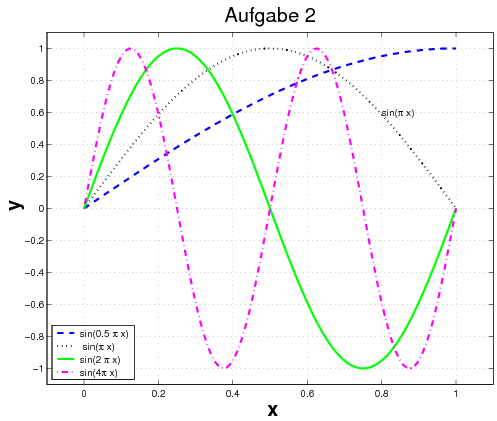
\includegraphics[width=0.6\textwidth]{../../figures/aufgabe2_24_11}\end{center}
\end{aufg}
%-----------------------------------------------------------------------------------
\begin{aufg}
Berechnen Sie $\int_0^1 xe^x dx$ exakt. Machen Sie die
  Probe, indem Sie das Programm \lstinline!integral.m! modifizieren. Wie
  groß muß $N$ mindestens gewählt werden, damit der absolute Fehler
  kleiner als $10^{-4}$ ist?
\end{aufg}
%-----------------------------------------------------------------------------------
\begin{aufg}
Stellen Sie die Funktion
\[ f(x,y,z)= \sin (4 \pi x) \sin( \pi y) y^2 (z^2-1), \quad (x,y,z) \in
[-1,1]^3 \]
grafisch dar.
\end{aufg}

-----------------------------------------------------------
\begin{aufg}
Seien $y_1,y_2$ zwei Punkte im $\mathbb{R}^2$. Wir betrachten die Strecke mit
Endpunkten $y_1$ und $y_2$. Wir ersetzen  diese Strecke durch 4 Strecken 
$\overline{y_1 z_1}$, $\overline{z_1 z_2}$, $\overline{z_2 z_3}$,
$\overline{z_3 y_2}$ mit Endpunkten $z_1=\frac23 y_1 + \frac13 y_2$,
$z_3=\frac13 y_1 + \frac23 y_2$ und 
\[ z_2 = \frac{\sqrt{3}}{6} \left( \begin{array}{cc}
0 & 1 \\ -1 & 0 \\
\end{array} \right)
(y_1 - y_2) + \frac12 (y_1 + y_2). \]
Analog zum Beispiel des Sierpinski-Dreiecks soll jede neue Teilstrecke
wiederum mittels der gleichen Prozedur durch 4 Strecken ersetzt werden. 
Schreiben Sie ein Programm, dass
diese Prozedur $k$-mal wiederholt und das Ergebnis plottet.
\end{aufg}


%-----------------------------------------------------------------------------------
\begin{aufg}
 Erstellen Sie eine Funktion, die zu einer gegebenen natürlichen
  Zahl $n$ ein regelmäßiges $n$-Eck zeichnet.\\

Wenden Sie auf die Kanten eines regelm\"a{\ss}igen Sechsecks, die rekursive
Funktion aus Blatt 2, Aufgabe 11 an.\\ 

{\it Hinweis:} Die Eckpunkte $(x_i,y_i)$ sind {
\[ x_i=\sin( 2 {\pi i}/{n} ), \quad  y_i=\cos( 2 {\pi i}/{n} ),
  \quad i=1, \dots ,n \]  }

\end{aufg}

%-----------------------------------------------------------------------------------
\begin{aufg}
Plotten Sie mit Hilfe von \lstinline!surf! die folgenden Funktionen auf
  $[-1,1]\times [-1,1]$
{
\[ \sin( \pi^2 xy), \ (x^2-1)(y^2-1), \ \sin(\pi x ^2), \ \sin(- \pi
  e^{-x^2-y^2}) \]}
in einem Grafikfenster (nicht ueberlappend). 
\end{aufg}

%-----------------------------------------------------------------------------------
\begin{aufg}
Plotten Sie die Funktion \[ f(x):= 1/(x^2+\sqrt{a}) \]
auf dem Intervall $[-3,3]$ f\"ur $a=1:20$ und erstellen Sie daraus eine Animation! 
\end{aufg}


%-----------------------------------------------------------------------------------


%Polynom-Aufgabe mit polyfit etc.!
%
%-------------------------------------------------------------------------------
\end{document}
%-------------------------------------------------------------------------------
